\documentclass{report}
\usepackage[utf8]{inputenc}
\usepackage{graphicx}
\usepackage{verbatim}

\title{Vienkāršu elektrisku shēmu modelēšana}
\author{Deniss Tiščenko }
\date{Marts 2019}

\begin{document}

\maketitle

\chapter{Teorētiskā daļa}

\section{Ķēdes aprēķins}
 Sprieguma avota V1 sprieguma vērtību U (Voltos) izvēlieties daļskaitli, kas būtu Jūsu apliecības pēdējie trīs cipari dalīti ar 10. Piemēram, ‘101REB123’ nozīmē V1 = 12.3 (Volti), R1 ir apliecības pēdējo 3 ciparu otrais numurs+1, R2 ir apliecības numura pēdējais cipars +1. Piemēram, ja Jūsu apliecības numurs ir ‘101REB123’ tad ‘R1=3’, ‘R2=4’.
\\
\\
UR1=V1*R1/(R1+R2)
\\
UR2=V1*R2/(R1+R2)
\\
\\
\begin{center}
\begin{tabular}{ | c | c | } 
\hline
R1 & 5 \\ 
\hline
R2 & 4 \\ 
\hline
V1 & 34,3 \\ 
\hline
UR2 & 19,06 \\ 
\hline
UR1 & 15,24 \\ 
\hline
\end{tabular}
\end{center}




\chapter{Praktiskā daļa}

\section{Darbs ar GEDA programmām}

\subsection{darbs ar gschem}
\begin{verbatim}
v 20130925 2
C 40000 40000 0 0 0 title-B.sym
C 47600 47300 1 0 0 resistor-2.sym
{
T 48000 47650 5 10 0 0 0 0 1
device=RESISTOR
T 48000 47600 5 10 1 1 0 0 1
refdes=R1
T 48000 47100 5 10 1 1 0 0 1
value=5
}
C 49500 46100 1 90 0 resistor-2.sym
{
T 49150 46500 5 10 0 0 90 0 1
device=RESISTOR
T 49200 46400 5 10 1 1 90 0 1
refdes=R2
T 49700 46500 5 10 1 1 90 0 1
value=4
}
N 46900 46700 46900 47400 4
{
T 47000 47100 5 10 1 1 270 0 1
netname=1
}
N 46900 47400 47600 47400 4
N 48500 47400 49400 47400 4
{
T 48900 47500 5 10 1 1 0 0 1
netname=2
}
N 49400 47400 49400 47000 4
N 46900 46000 46900 45700 4
N 46900 45700 49400 45700 4
{
T 48200 45500 5 10 1 1 0 0 1
netname=0
}
N 49400 45700 49400 46100 4
C 46700 46700 1 270 0 battery-1.sym
{
T 47600 46400 5 10 0 0 270 0 1
device=BATTERY
T 47200 46700 5 10 1 1 270 0 1
refdes=V1
T 48000 46400 5 10 0 0 270 0 1
symversion=0.1
T 47200 46400 5 10 1 1 270 0 1
value=34.3
}
\end{verbatim}

\subsection{darbs ar gnetlist}
\begin{verbatim}
* Spice netlister for gnetlist
V1 1 0 34.3
R2 0 2 4
R1 1 2 5
.END
\end{verbatim}

\subsection{darbs ar ngspice}
\rotatebox{-90}{\includegraphics[width=10cm]{01.ps}}

\section{Darbs ar QUCS programmām}
\subsection{Principāla shēma un līdzstrāvas simulācijas (DC simulation) grafiks}
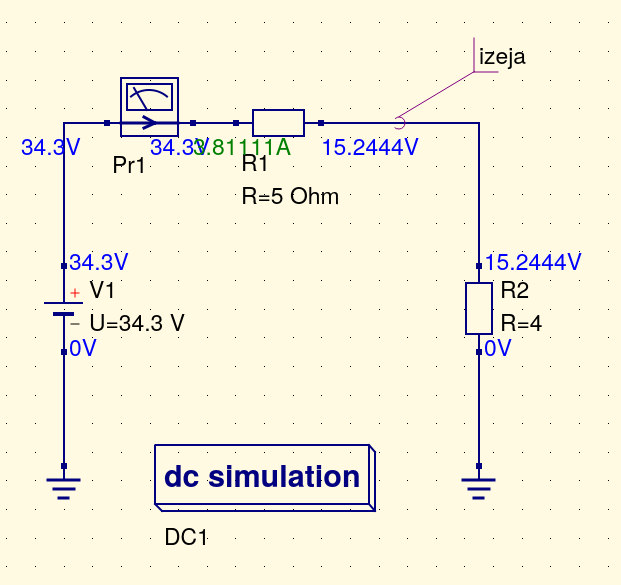
\includegraphics[width=15cm]{shema.png}

\subsection{Sweep simulācijas grafiks un tabula}
\rotatebox{-90}{\includegraphics[width=40cm]{02.ps}}

\end{document}
